\subsection*{1.}
می‌دانیم:
\begin{figure}[H]
    \centering
    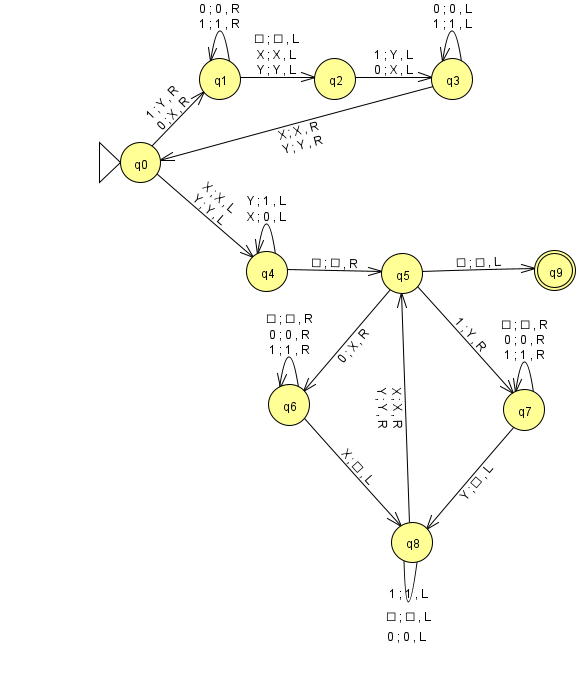
\includegraphics[scale=0.7]{solution/1-1.png}
\end{figure}

با فرض 
$r > k$ داریم:
\begin{center}
    \[ \lim_{n\to\infty} \frac{n^k}{n^r} \]  =  \[ \lim_{n\to\infty} \frac{1}{n^{r-k}} \]  =
    0
\end{center}
در نتیجه اثبات شد.

\subsection*{2.}
داریم:
\begin{center}
    \begin{itemize}
        \item 
        $\forall f(n) \in  O(\log(n)): 
        \exists c, n_0\; s.t.\; \forall \; n \geq n_0:\; f(n) \leq 
        c.\log(n)\; \rightarrow \; \frac{f(n)}{\log(n)} \leq c
        \; \rightarrow \frac{f(n)}{\log(n)}\;\in\; O(1)\;
        \Longrightarrow \; f(n)\;\in\; O(1)\log(n)$ 
        \item 
        $\forall f(n) \in O(1)\log(n): 
        \exists c, n_0\; s.t.\; \forall \; n \geq n_0:\; f(n) \leq 
        \log(n)*1*c\; \rightarrow \; f(n) \leq c.\log(n)\;
        \Longrightarrow \; f(n)\;\in\;O(\log(n))$
    \end{itemize}
\end{center}
در نتیجه:
\begin{center}
    $O(\log(n)) = O(1)\log(n)$
\end{center}
سپس:
\begin{center}
    $O(\log(n)) = O(1)\log(n) \Longrightarrow\;
    2^{O(\log(n))} = 2^{O(1)\log(n)} = n^{O(1)}$
\end{center}
دقت کنید می‌دانیم که 
$n = 2^{\log(n)}$.

\subsection*{3. }
ابتدا به راه سورس درس برای این سوال نگاه می‌کنیم:
\begin{figure}[H]
    \centering
    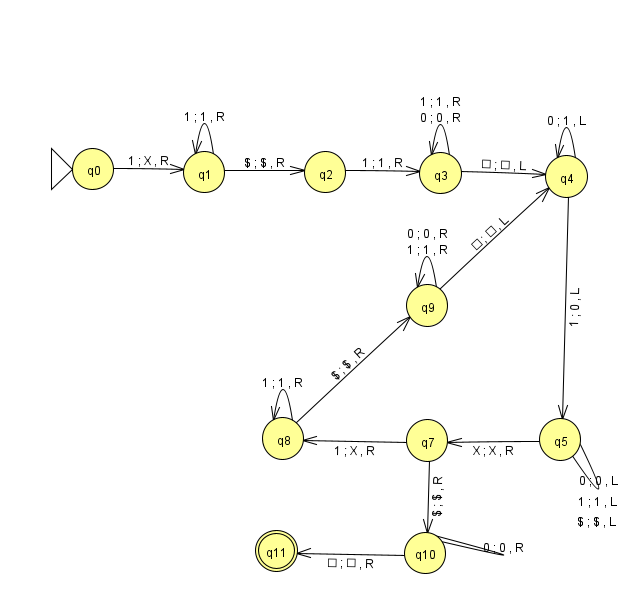
\includegraphics[scale=1.1]{solution/1-2.png}
\end{figure}
حال راه خود را ارائه می‌کنیم:\\
مااند بخش اول داریم:
\begin{center}
    \[ \lim_{n\to\infty} \frac{2^n}{3^n} \] = \[ \lim_{n\to\infty} (\frac{2}{3})^n \] $= 0$
\end{center}
به بیان دیگر:
\begin{center}
    $2^n < c * 3^n$\\
    $\frac{1}{c} < \frac{3^n}{2^n} = (1.5)^n  \;\Leftrightarrow\;
    \log_{1.5}(\frac{1}{c}) < n$\\
    $\rightarrow \; n_0 \leq \log_{1.5}(\frac{1}{c})$ \\
    \lr{\text{for} $n > n_0$, \text{we have} $n > n_0 > \log_{1.5}(\frac{1}{c})$}
\end{center}